%%%%%%%%%%%%%%%%%%%%%%%%%%%%%%%%%%%%%%%%%
% Beamer Presentation
% LaTeX Template
% Version 1.0 (10/11/12)
%
% This template has been downloaded from:
% http://www.LaTeXTemplates.com
%
% License:
% CC BY-NC-SA 3.0 (http://creativecommons.org/licenses/by-nc-sa/3.0/)
%
%%%%%%%%%%%%%%%%%%%%%%%%%%%%%%%%%%%%%%%%%

%----------------------------------------------------------------------------------------
%   PACKAGES AND THEMES
%----------------------------------------------------------------------------------------

\documentclass[xcolor=table]{beamer}

\mode<presentation> {

%dencoding
%--------------------------------------
\usepackage[utf8]{inputenc}
\usepackage[T1]{fontenc}
%--------------------------------------

%Portuguese-specific commands
%--------------------------------------
\usepackage[portuguese]{babel}
%--------------------------------------

%Hyphenation rules
%--------------------------------------
\usepackage{hyphenat}
\hyphenation{mate-mática recu-perar}
%--------------------------------------

%--------------------------------------
\usepackage{textpos}
%--------------------------------------
\fboxsep0pt
%--------------------------------------

% --verticalmente centralizado----
\usepackage{array,booktabs}% http://ctan.org/pkg/{array,booktabs}
\usepackage{multirow}
% ---------------


\bibliographystyle{plain}

% The Beamer class comes with a number of default slide themes
% which change the colors and layouts of slides. Below this is a list
% of all the themes, uncomment each in turn to see what they look like.

%\usetheme{default}
%\usetheme{AnnArbor}
%\usetheme{Antibes}
%\usetheme{Bergen}
%\usetheme{Berkeley}
%\usetheme{Berlin}
%\usetheme{Boadilla}
%\usetheme{CambridgeUS}
%\usetheme{Copenhagen}
%\usetheme{Darmstadt}
%\usetheme{Dresden}
%\usetheme{Frankfurt}
%\usetheme{Goettingen}
%\usetheme{Hannover}
%\usetheme{Ilmenau}
%\usetheme{JuanLesPins}
%\usetheme{Luebeck}
%\usetheme{Madrid}
%\usetheme{Malmoe}
%\usetheme{Marburg}
\usetheme{Montpellier}
%\usetheme{PaloAlto}
%\usetheme{Pittsburgh}
%\usetheme{Rochester}
%\usetheme{Singapore}
%\usetheme{Szeged}
%\usetheme{Warsaw}


% As well as themes, the Beamer class has a number of color themes
% for any slide theme. Uncomment each of these in turn to see how it
% changes the colors of your current slide theme.

%\usecolortheme{albatross}
%\usecolortheme{beaver}
%\usecolortheme{beetle}
\usecolortheme{crane}
%\usecolortheme{dolphin}
%\usecolortheme{dove}
%\usecolortheme{fly}
%\usecolortheme{lily}
%\usecolortheme{orchid}
%\usecolortheme{rose}
%\usecolortheme{seagull}
%\usecolortheme{seahorse}
%\usecolortheme{whale}
%\usecolortheme{wolverine}

%\setbeamertemplate{footline} % To remove the footer line in all slides uncomment this line
\setbeamertemplate{footline} % To replace the footer line in all slides with a simple slide count uncomment this line

\setbeamertemplate{footline}{
\leavevmode%
  \hbox{%
  \begin{beamercolorbox}[wd=.4\paperwidth,ht=2.25ex,dp=1ex,center]{author in head/foot}%
    \usebeamerfont{author in head/foot}\insertshortauthor
  \end{beamercolorbox}%
  \begin{beamercolorbox}[wd=.6\paperwidth,ht=2.25ex,dp=1ex,center]{title in head/foot}%
    \usebeamerfont{title in head/foot}\insertshorttitle\hspace*{6em}
    \insertframenumber{} / \inserttotalframenumber\hspace*{1ex}
  \end{beamercolorbox}}%
  \vskip0pt
}

\setbeamertemplate{navigation symbols}{} % To remove the navigation symbols from the bottom of all slides uncomment this line
}

\usepackage{graphicx} % Allows including images
\graphicspath{ {./imagens/} }
\usepackage{booktabs} % Allows the use of \toprule, \midrule and \bottomrule in tables

% letras riscadas em cima
\usepackage[normalem]{ulem}

% -----------------------------------------------------
% descomente essa seção para habilitar o logo da utfpr
% (talvez o tamanho e o local devem ser alterados para
% caber no cabeçalho)
%
% \addtobeamertemplate{frametitle}{}{%
% \begin{textblock*}{100mm}(0.85\textwidth,-1.9cm)
% 
\includegraphics[height=.1\textwidth]{./imagens/utfpr-logo.png}
% \end{textblock*}
% }
% -----------------------------------------------------

%%----------------------------------------------------------------------------------------
%   TITLE PAGE
%----------------------------------------------------------------------------------------

%--------------------------------------
\title[Defesa de Proposta de TCC]{Aplicação do Processo de Descoberta de Conhecimento em Bases de Dados de Domínios Públicos} % The short title appears at the bottom of every slide, the full title is only on the title page

\author[Gabriel]{
Gabriel Levis Zawalski\\ \footnotesize Orientadora: Profª Helyane Bronoski Borges \\ \footnotesize Coorientadora: Thissiany Beatriz Almeida
} % Your name

\institute[UTFPR] % Your institution as it will appear on the bottom of every slide, may be shorthand to save space
{
Universidade Tecnológica Federal do Paraná\\ % Your institution for the title page
\medskip
\textit{gabrielzawalski@gmail.com} \\ % Your email address
\medskip
\url{https://github.com/glzawalski/} 
}
\date{\today} % Date, can be changed to a custom date

% numerais romanos
\makeatletter
\newcommand*{\rom}[1]{\expandafter\@slowromancap\romannumeral #1@}
\makeatother
\begin{document}

\begin{frame}
\titlepage % Print the title page as the first slide
\end{frame}

%----------------------------------------------------------------------------------------
%   PRESENTATION SLIDES
%----------------------------------------------------------------------------------------

% SUMÁRIO----------------------------------------------------------------------

\renewcommand{\contentsname}{SUMÁRIO}

\pdfbookmark[0]{\contentsname}{toc}
\tableofcontents*
\cleardoublepage

% OBSERVAÇÕES-------------------------------------------------------------------
% Este arquivo não precisa ser alterado, pois o sumário é gerado automaticamente.

\section{Introdução}

\subsection{Contexto}
\begin{frame}
	\begin{itemize}
		\item Aumento da presença de serviços digitais na vida cotidiana;
		\item Acumular dados não é o suficiente;
		\item Métodos tradicionais de análise estatística requerem interpretação manual;
		\item Fayyad 1996 \cite{fayyad1996} diz que neste cenário há uma grande necessidade de novas teorias e ferramentas computacionais a fim de auxiliar na extração de conhecimento dos grandes e cada vez maiores volumes de dados.
	\end{itemize}
\end{frame}

\subsection{Processo de KDD}

\begin{frame}
	\begin{itemize}
		\item Knowledge Discovery in Databases - cunhado por Shapiro em 1989;
		\item Processo iterativo e não trivial dependente de interações do usuário;
		\item Tem como objetivo identificar informações válidas, novas, potencialmente úteis e compreensíveis em um grupo de dados.
	\end{itemize}
\end{frame}

\begin{frame}
	\begin{figure}[h!]
		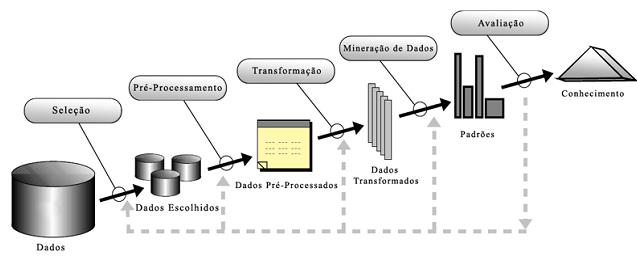
\includegraphics[width=\textwidth]{KDD}
		\caption{Fluxograma do processo de KDD. Adaptado de Fayyad 1996 \cite{fayyad1996}.}
	\end{figure}
\end{frame}

\begin{frame}
	\begin{itemize}
		\item A mineração de dados é uma das etapas do KDD que mais recebe destaque;
		\item Grande quantidade de técnicas e resultados disponíveis para teste;
		\item Descoberta e adaptação de padrões e modelos;
		\item Classificação, Clusterização e Regressão.
	\end{itemize}
\end{frame}
\section{Obejtivos}

\subsection{Objetivos Gerais}
\begin{frame}
	\begin{itemize}
		\item O objetivo geral deste trabalho é aplicar o processo de KDD numa base de dados de domínio público a fim de criar um modelo de previsão de sucesso de postagem.
	\end{itemize}
\end{frame}

\subsection{Objetivos Específicos}
\begin{frame}
	\begin{enumerate}
		\item Compreender o funcionamento do processo de KDD;
		\item Analisar as etapas do KDD, identificado técnicas que podem ser aplicadas;
		\item Aplicar o processo de KDD na base de dados;
		\item Realizar experimentos e analisar os resultados obtidos através de comparação estatística com outros trabalhos da área.
	\end{enumerate}
\end{frame}
\section{Justificativa}

\begin{frame}
	\begin{itemize}
		\item Possuir dados não siginfica ter algum conhecimento;
		\item Sem análise rigorosa conclusões erradas podem ser tomadas;
		\item KDD se torna interessante pois estabelece um processo de fácil replicação;
		\item A base de dados escolhida possui dados reais e recentes.
	\end{itemize}
\end{frame}
% METODOLOGIA------------------------------------------------------------------

\chapter{METODOLOGIA}
\label{chap:metodologia}
Metodologia, ferramenta e base utilizada na pesquisa.

\section{PRÉ-PROCESSAMENTO}
\label{sec:metodologiaPreProc}
Tudo que foi aplicado na base de dados.

\section{MINERAÇÃO DE DADOS}
\label{sec:metodologiaMine}
Tudo que foi aplicado para mineração, svm e regressão.

\section{PÓS-PROCESSAMENTO}
\label{sec:metodologiaPosProc}
Tudo que foi feito após o proc de datamining.
\section{Cronograma}

\begin{frame}
	placeholder quadro de cronograma.
\end{frame}
% REFERÊNCIAS------------------------------------------------------------------

% Carrega o arquivo "base-referencias.bib" e extrai automaticamente as referências citadas

\bibliography{./base-referencias}
\bibliographystyle{abntex2-alf} % Define o estilo ABNT para formatar a lista de referências
% OBSERVAÇÕES------------------------------------------------------------------
% Este arquivo não precisa ser alterado.


%------------------------------------------------

\section*{}
\begin{frame}
\titlepage
\end{frame}

%----------------------------------------------------------------------------------------
\end{document}
